The forward models in Chapter~\ref{ch:results} are trained and tested on frequencies drawn from the same 10 to 160\,Hz band, so a good test-split score only shows that a model can interpolate between frequencies it has already seen. A separate, smaller experiment checks a stricter question: can a model also handle a band of frequencies it never saw at all during training? This is kept out of the main results because it uses an earlier, 3-resonator dataset of 10{,}000 configurations rather than the 2-resonator, 5-variable dataset used everywhere else in this thesis, and because it only answers a secondary question about extrapolation, not the generative-design objective of the thesis.

\section{Setup}

The middle 20\,\% of the frequency band, 70 to 100\,Hz, is removed completely from training and validation: the models never see a solver spectrum value inside this band while learning. After training, each model is evaluated on the full band and scored separately on the frequencies it trained on (``seen'') and the held-out band (``unseen''). A large gap between the two scores means a model has mostly memorised input-output pairs at the frequencies it was shown, rather than learning the underlying physics well enough to fill in a gap.

Six of the ten architectures from Chapter~\ref{ch:results} are included in this experiment: DON, DNO, DCO, WNO, GNO and NN.

\section{Results}

\begin{table}[h]
\centering
\caption[Seen vs. unseen RMSE in the frequency-holdout experiment]{Root-mean-square error (RMSE), mean absolute error (MAE) and Pearson correlation on the seen frequencies versus the held-out 70--100\,Hz band.}
\begin{tabular}{lrrrrrr}
\hline
Model & RMSE seen & RMSE unseen & MAE seen & MAE unseen & $r$ seen & $r$ unseen \\
\hline
DNO & 3.98 & 7.11 & 1.95 & 4.45 & 0.922 & 0.544 \\
DCO & 3.95 & 7.38 & 1.94 & 4.83 & 0.924 & 0.521 \\
NN  & 4.88 & 7.17 & 2.86 & 4.72 & 0.880 & 0.493 \\
GNO & 4.10 & 7.67 & 2.11 & 4.99 & 0.917 & 0.439 \\
WNO & 5.59 & 8.92 & 3.07 & 6.39 & 0.840 & 0.258 \\
DON & 6.35 & 13.37 & 3.93 & 10.31 & 0.812 & 0.125 \\
\hline
\end{tabular}
\end{table}

Every model is clearly worse on the held-out band: RMSE roughly doubles to triples, and the Pearson correlation on the unseen band drops well below the seen-band value for every architecture. DNO and DCO cope best with the gap, while DON is affected the most. Figure~\ref{fig:holdout-example} shows one example spectrum from this experiment: the solver curve and the model prediction agree closely outside the grey band, but the model prediction departs from the solver curve inside it.

\begin{figure}[h]
\centering
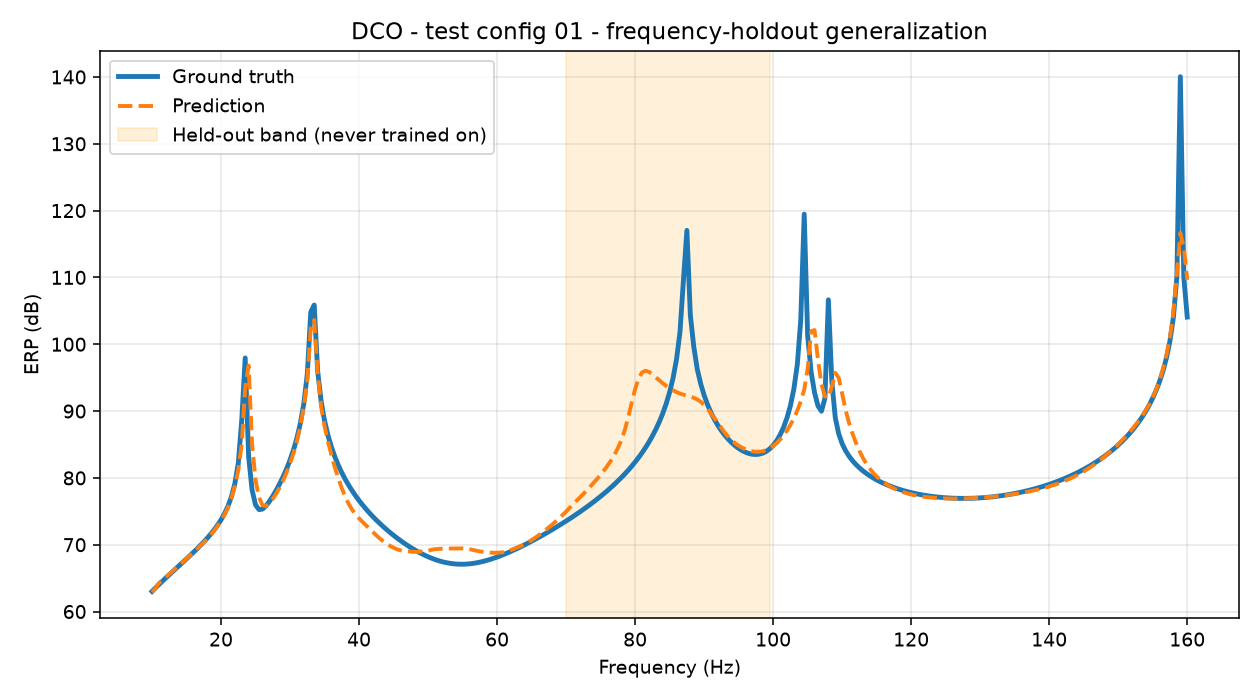
\includegraphics[width=0.85\textwidth]{Bilder/holdout_example.png}
\caption[Example spectrum from the frequency-holdout experiment]{Example test spectrum from the frequency-holdout experiment. The model was never trained on the shaded 70--100\,Hz band.}
\label{fig:holdout-example}
\end{figure}

The practical conclusion is simple: these forward surrogates are reliable for interpolating within the frequency band they were trained on, which is exactly how they are used in this thesis, but they should not be trusted to extrapolate to frequencies outside their training range without retraining on data that covers that range.
